
In this subsection, we relate the free energy to the amplitudes between boundary states and present the analytic results. 

We notice that there is only one apparent length scale in these diagrams -- the finite size $L$ for fidelity and imaginary time $\tau$ for the Loschmidt echo. These are the characteristic size of the corners at the tip of the slits. Regulators are necessary in keeping track of the scale dependence, otherwise a dilation transformation can rescale both $L$ and $\tau$ to $1$ and drop those scales. The introduction of regulators is also physically sensible when considering the lattice realization of the systems. 

We thus add small semi-circles around the points where the bcc operators reside, and then apply a series of conformal mappings. 

For the fidelity case, the regulators as well as the conformal maps are depicted in Fig.~\ref{fig:fidel-map}. 
\begin{figure}[h]
\centering
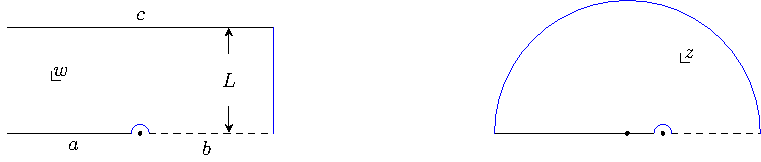
\includegraphics[width=\columnwidth]{fig_fidel-map.pdf}
\caption{Mapping from a strip to the upper half plane $\xi  = \exp( \frac{\pi z}{L} ) $. The two black dots represent possible locations of boundary condition changing (bcc) operators. The dot inside the blue semi-circle has coordinate $\xi = 1$, which is the image of the point connecting $a$ and $b$ boundaries. The other dot $\xi = 0$ corresponds to the connection between $a$ and $c$ boundaries at $- \infty$. To evaluate the diagram, we add the outer blue semi-circle centered at $\xi = 1$ with radius $R_{\xi}$ to be the IR cut-off and map it to the cylinder with $w = \ln(\xi - 1)$}
\label{fig:fidel-map}
\end{figure}
We add a small blue semi-circle to the folded strip in Fig.~\ref{fig:fidel} as the UV regulator and map it to the upper half plane using $\xi  = \exp( \frac{\pi z}{L} )$. Then both $\xi = 0$ and $1$ can host bcc operators. We assume $a = c$ such that the only bcc operator on the real axis is the one enclosed by the blue semi-circle around $\xi = 1$. In order to evaluate this diagram, we add another semi-circle centered around $\xi = 1$ with radius $R_{\xi}$ (this will introduce a correction as explained in App.~\ref{app:F_correction}), and map it to a cylinder of height $\pi$ on the right by $w = \ln ( \xi- 1)$. Finally the cylinder diagram can be viewed as an imaginary time path integral amplitude between the boundary states $b$ and $a$
\begin{equation}
\label{eq:partition_fun}
Z_{ab} = \langle a | e^{-\pi H } |b \rangle.
\end{equation}
The two end points of the $\epsilon$ radius semi-circle on the $z$ plane are mapped to
\begin{equation}
\exp( \pm \pi \frac{\epsilon}{ L}  ) \sim 1 \pm \pi \frac{\epsilon}{L} .
\end{equation}
The bigger blue semi-circle intersects the real axis at $1 \pm R_{\xi}$ and so the width of the cylinder is 
\begin{equation}
\label{eq:fidel_cyd_width}
\ln R_{\xi} - \ln \frac{\pi \epsilon}{L} = \ln L + \text{constant}.
\end{equation}

The Loschmidt echo can be evaluated in the same way. Again, we introduce two semi-circles (blue in Fig.~\ref{fig:H-tau_fold}) as regulators and then perform the conformal transformation shown in Fig.~\ref{fig:H-tau_fold}. From $z$ plane to the $\xi$ plane, we use $\xi = \frac{z}{\tau - z}$ to map the two slits to half of an annulus, which is the same as the fidelity case. With one more conformal mapping $w = \ln \xi$, the diagram again becomes the cylinder partition function between the two boundary states. 

The height of the cylinder is still $\pi$. In the $\xi$ plane, the coordinates of the two end points of the small semi-circle are $\frac{\pm \epsilon}{ \tau \mp \epsilon} \sim \frac{\pm \epsilon}{ \tau }$, while those of the larger semi-circle are $\mp \frac{\tau \pm \epsilon}{\epsilon} \sim \frac{\mp \tau}{\epsilon}$. Hence the width of the cylinder is
\begin{equation}
\label{eq:echo_cyd_width}
\ln \frac{\tau}{\epsilon} - \ln \frac{\epsilon}{\tau } = 2 \ln \tau + \text{constant}.  
\end{equation}

\begin{figure}[htb]
\centering
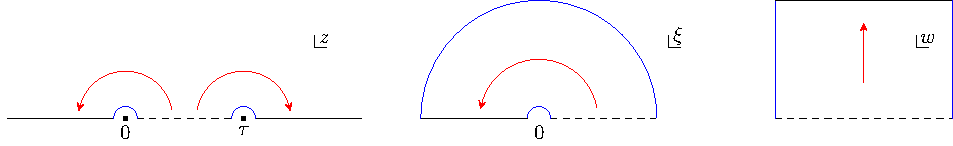
\includegraphics[width=\columnwidth]{fig_H-tau_fold}
\caption{The dashed (solid) lines are gluing (completely reflective) boundary conditions. Red arrows are the directions of Hamiltonian flow that propagates the dashed line boundary state to the solid line boundary state. Left: Diagram of the Loschmidt echo that reduces to a partition function with imaginary time in the horizontal direction. The blue semi-circles of radius $\epsilon$ are the UV regulators and they are identified as periodic boundaries in the direction perpendicular to the red arrow (equal time slice). Middle: Image of the map $\xi = \frac{z}{\tau - z}$. The two semi-circles have radii $({\tau}/{\epsilon})^{\pm1}$ respectively.  Right: Image of $w = \ln \xi$. It is a cylinder by identifying the blue lines and the standard radial quantization procedure can be applied. }
\label{fig:H-tau_fold}
\end{figure}


One subtlety of the above description is that the two semi-circles in the center diagrams of Fig.~\ref{fig:fidel-map} and Fig.~\ref{fig:H-tau_fold} are not precisely concentric. This can be resolved by the following observation. There exists conformal map $\zeta(\xi)$ that maps the non-concentric circles to two standard concentric circles of radii $1$ and $R$ ($R>1$) on the $\zeta$ plane\cite{brown_complex_2009}. Then the logarithmic map $w = \ln \zeta$ produces a cylinder of width $\ln R$. In our case, since the height of the cylinder is always $\pi$, the width of the cylinder is a conformal invariant that only depends on the cross ratio of the half annulus. The four intersection points of two standard concentric circles on $\zeta$ plane are $(\pm 1,0)$ and $(\pm R,0)$, whose cross ratio is
\begin{equation}
\eta = \frac{(1 + R)^2}{(1 - R)^2}. 
\end{equation}
Hence the width of the cylinder is $\ln \frac{\sqrt{ \eta } - 1}{\sqrt{ \eta} + 1}$. Since conformal transformation preserves the cross ratio, the result is the same if we use the cross ratio of the slightly non-concentric diagrams of Fig.~\ref{fig:fidel-map} and Fig.~\ref{fig:H-tau_fold}. The calculation in Eq.~\eqref{eq:fidel_cyd_width} and Eq.~\eqref{eq:echo_cyd_width} equivalently use the leading order approximation to $\eta$ in the respective geometries and thus get the leading order term in the width of the cylinders. The slight deviation to the precise concentric geometry will only bring in $\frac{\epsilon}{L}, \frac{\epsilon}{\tau}$ corrections to $\eta$ and the width parameter, so will not affect the fidelity and echo exponents. 

For the rest of this section, we should denote the width of the cylinder as $\beta$. After obtaining the partition function on it, we should set $\beta = 2 \ln L$ or $ 4 \ln \tau$ because the fidelity and Loschmidt echo are both square of the amplitudes.

The actual boundary conditions on the blue lines, which are the regulators in Fig.~\ref{fig:fidel-map} and Fig.~\ref{fig:H-tau_fold}, are not important in the leading order. Taking Fig.~\ref{fig:fidel-map} for example, rather than using Eq.~\eqref{eq:partition_fun}, we can alternatively view the right panel as the amplitude between the two blue boundary states $|1\rangle$ and $|2\rangle$
\begin{equation}
Z_{ab} =  \langle 1 | e^{ - \beta H_{ab}} | 2 \rangle  , 
\end{equation}
where $H_{ab}$ is the Hamiltonian with boundary condition $a$ and $b$. Since $\beta$ is taken to be large, we expect the imaginary time evolution (which is horizontal in this case) to project out only the groundstate $|0_{ab}\rangle $. Hence the free energy is
\begin{equation}
\begin{aligned}
F &=  - \ln Z_{ab}  \sim - \ln \langle 1 |0_{ab} \rangle \langle   0_{ab}  |e^{ - \beta H_{ab}}|0_{ab} \rangle \langle 0_{ab} | 2 \rangle \\
&= \beta  E_c - \ln \langle 1| 0_{ab} \rangle  - \ln \langle 0_{ab}  |2 \rangle,
\end{aligned}
\end{equation}
where $E_c$ is the groundstate/Casimir energy of $H_{ab}$. We see that different choices of the boundary conditions only change the term independent of $\beta$. Thus in the leading order we can choose any boundary conditions. The one we pick is the simplest one: the periodic boundary condition that identifies the two blue lines. 

With these simplifications, we now set up the partition function calculation of the general process $S_a( \theta_1 ) \rightarrow S_b( \theta_2)$. We define a set of bosonic operators related to the $a^i_n$s in Eq.~\eqref{eq:di_mode_expansion} through
\begin{equation}
\begin{aligned}
b^i_n &= \frac{a^i_n}{\sqrt{n}} \quad (b^i_n)^{\dagger} &= \frac{a^i_{-n}}{\sqrt{n}} \\
\bar{b}^i_n &= \frac{\bar{a}^i_n}{\sqrt{n}} \quad (\bar{b}^i_n)^{\dagger} &= \frac{\bar{a}^i_{-n}}{\sqrt{n}} \\
\end{aligned}
\end{equation}
for $n > 0 , i = 1, 2$, and group them compactly with the vector notation
\begin{equation}
\begin{aligned}
\vec{b}_i &= ( b^i_1, b^i_2, \cdots )^\top, \qquad \,\,\quad \vec{\bar{b}}_i = ( \bar{b}^i_1, \bar{b}^i_2, \cdots )^\top\\
\vec{b}^\dagger_i &= ( (b^i_1)^\dagger, (b^i_2)^\dagger, \cdots )^\top, \quad\vec{\bar{b}}^{\dagger}_i = ( (\bar{b}^i_1)^\dagger, (\bar{b}^i_2)^\dagger, \cdots )^\top.
\end{aligned}
\end{equation}
The boundary state in Eq.~\eqref{eq:bd_state} is then 
\begin{equation}
\exp\Big\{  (\vec{b}_1^{\dagger} \vec{b}_2^{\dagger} ) R_a( \theta )   
\begin{pmatrix}
  \vec{\bar{b}}_1^{\dagger}\\
  \vec{\bar{b}}_2^{\dagger}
\end{pmatrix}\Big\}  |0  \rangle ,
\end{equation}
where $R_a( \theta ) = -S_a \otimes \mathbb{I}$. Using even a lazier notation $\vec{b} = ( \vec{b}_1, \vec{b}_2 )^\top$, we have
\begin{equation}
\label{eq:bd_state_matrix}
|a \rangle = \exp\Big\{  \vec{b}^{\dagger} R_a( \theta )    \vec{\bar{b}}^{\dagger} \Big\} |0 \rangle .
\end{equation}
The matrix notation here should be understood as a bilinear expression. For example, $\vec{b}^{\dagger} R \bar{\vec{b}}^{\dagger}$ actually means $\sum_{ij}b^\dagger_iR_{ij}\bar{b}_j^\dagger$ where the dagger does not transpose the vector.

The Hamiltonian of the folding picture has the mode expansion in terms of the $b_n$ (with periodic boundary conditions)
\begin{equation}
\begin{aligned}
  H &= \frac{2\pi}{\beta} (L_0 + \bar{L}_0) =  \frac{4\pi}{\beta}  L_0 \\
  &= \frac{4\pi}{\beta}\sum_{\substack{n > 0\\ i=1,2} }  n (b^i_n)^{\dagger} b^i_n \\
  &=  \frac{1}{\pi}(\vec{b}_1^{\dagger} \vec{b}_2^{\dagger} ) (\mathbb{I}_2  \otimes M)
\begin{pmatrix}
  \vec{{b}_1}\\
  \vec{{b}_2}
\end{pmatrix}\\
 &= \frac{1}{\pi} \vec{b}^{\dagger}  (\mathbb{I}_2  \otimes M)  \vec{b} ,
\end{aligned}
\end{equation}
where $L_0+ \bar{L}_0$ are the dilation operator in CFT and we have used the condition $L_0 = \bar{L}_0$ when restricted to the space of the boundary states. The infinite dimensional matrix $M$ is
\begin{equation}
M =  \frac{4\pi^2}{\beta} \text{diag}( 1, 2, \cdots ).
\end{equation}
The partition function in Eq.~\eqref{eq:partition_fun} becomes
\begin{equation}
\label{eq:Zab-bd}
\begin{aligned}
Z_{ab} =& \langle b | e^{-\pi H} | a \rangle \\
=& \langle 0 | \exp\Big\{  \vec{b} R_b( \theta )    \vec{\bar{b}} \Big\}  \exp\Big\{ -\vec{b}^{\dagger}  (\mathbb{I}_2  \otimes M)  \vec{b} \Big\} \\
&\exp\Big\{  \vec{b}^{\dagger} R_a( \theta )    \vec{\bar{b}}^{\dagger} \Big\} | 0\rangle .
\end{aligned}
\end{equation}

In App.~\ref{app:lambda_12}, we obtained the leading order term in the free energy associated with Eq.~\eqref{eq:Zab-bd}. This expression is also obtained by an alternative Casimir energy calculation in App.~\ref{app:gnd_dn_lambda} for one set of the boundary conditions. A na\"ive application of the result however will lead to an apparent contradiction. One notable example is that when $a = b  = {\rm P}$, the free energy given by App.~\ref{app:lambda_12} is $- \frac{1}{12}\beta$, which should actually be {\it zero} because this is the (regularized) free energy on a plane without any interface. Physically this corresponds to the situation that the boundary condition does not change after joining the two chains. Hence the Loschmidt echo will stay at $1$ and the free energy is $0$. This motivates a shift to the free energy
\begin{equation}
\mathcal{F} = - \ln Z_{ab} ( \beta ) + \frac{1}{12} \beta ,
\end{equation}
where $\frac{1}{12}\beta$ is the value of $ \ln Z_{ab} ( \beta )$ when $a = b = {\rm P}$. A more careful inspection in App.~\ref{app:F_correction} shows the origin of the shift: part of it comes from the outer semi-circles in the middle panel of Fig.~\ref{fig:fidel-map} and Fig.~\ref{fig:H-tau_fold}, and another part comes from the non-homogeneous term in the conformation transformation of the stress tensor from annulus to cylinder. 

After incorporating this shift, for the process ($c$ is assumed to be the same as $a$)
\begin{equation}
\label{eq:S_i_S_j}
S_i( \theta_1 ) \rightarrow S_j( \theta_2 ) ,
\end{equation}
the free energy is
\begin{equation}
\mathcal{F}( \beta )  = 
\left\lbrace
\begin{aligned}
  &\frac{1}{2}(|x| - x^2 )\beta  \quad &i = j \\
  &\frac{1}{16}\beta   \quad &i \ne j ,  \\
\end{aligned} \right. \quad x = \frac{\theta_2 - \theta_1}{\pi} .
\end{equation}
We can then set $\beta = 2 \ln L$ and $ 4 \ln t$ (after analytic continuing to real time) to get the fidelity and echo exponent. 

As analyzed in Sec.~\ref{sec:analytic_numerics}, $S_2( \theta)$ interpolates between DD and NN, $S_1( \theta )$ interpolates between DN and ND. In the region accessible to the numerical calculation in the lattice model, we choose the process ${\rm DD} \rightarrow  \lambda$ to verify
\begin{equation}
\label{eq:result_DDDD}
\mathcal{F} = 
\left\lbrace
\begin{aligned}
\frac{1}{8}\ln L  &\quad\text{fidelity}  \\
\frac{1}{4}\ln t   &\quad \text{echo} .  \\
\end{aligned} \right.  
\end{equation}
The same results have already been obtained for $\lambda = {\rm P}$\cite{stephan_logarithmic_2013,stephan_local_2011,vasseur_universal_2014,vasseur_crossover_2013,kennes_universal_2014}. Another process $\rm{DN} \rightarrow \lambda$ {\iffalse \color{red} in Eq.~\eqref{eq:DNDN}\fi} is used to verify
\begin{equation}
\label{eq:result_DNDN}
\mathcal{F} = 
\left\lbrace
\begin{aligned}
 (x - x^2 )\ln L   &  \quad {\rm fidelity} \\
 2(x - x^2 ) \ln t  & \quad \text{ Loschmidt echo} , \\
\end{aligned} \right. 
\end{equation}
where $\lambda = \tan \theta$ and $x = \frac{\theta}{\pi}$. 

We also use a more artificial process ${\rm P} \rightarrow \lambda$ to check the shift of the curve
\begin{equation}
\label{eq:periodic-case}
\mathcal{F} = 
\left\lbrace
\begin{aligned}
  \Big(|x-\frac{1}{4}| - (x-\frac{1}{4})^2 \Big)\ln L   &  \quad {\rm fidelity} \\
  2\Big(|x-\frac{1}{4}| - (x-\frac{1}{4})^2 \Big) \ln t  & \quad \text{ Loschmidt echo} .\\
\end{aligned} \right. 
\end{equation}



%%% Local Variables:
%%% TeX-master: "bCFT_paper"
%%% TeX-PDF-mode: t
%%% End:
